%Vorlage
\documentclass[12pt,a4paper]{scrartcl}
\usepackage[english]{babel} %Für die indirekte Angabe von Umlauten. Es müssen dann Umlaute wie folgt im Code angegeben werden: "a "o "u "s.

\usepackage[utf8]{inputenc}
%Math
\usepackage{amsmath, amsthm, amssymb}
\usepackage{braket}
\newcommand{\tens}[1]{% https://tex.stackexchange.com/questions/171788/always-have-the-ring-of-the-tensor-product-below-the-otimes -> Tensor Product
  \mathbin{\mathop{\otimes}\displaylimits_{#1}}%
}
%Page numbers
\usepackage{enumerate}
%Graphics
\usepackage{graphicx}
\usepackage{floatrow}
\graphicspath{{./images/}}
%Quantum circuits http://mirrors.ibiblio.org/CTAN/graphics/pgf/contrib/quantikz/quantikz.pdf
\usepackage{tikz}
\usetikzlibrary{quantikz}
\usepackage{lscape}
\usepackage{setspace}
\onehalfspacing
\usepackage{wrapfig}
\usepackage{hyperref}% für die Einbettung von Hyperlinks
\def\UrlBreaks{\do\/\do-}
\usepackage{multirow}
\usepackage{csquotes} %Quotations


% Margins
%\usepackage{geometry} % Document Margins
%\setlength{\topmargin}{0cm}
%\setlength{\parindent}{5mm}
%\setlength{\parskip}{2mm}
%\setlength{\evensidemargin}{0mm}
%\setlength{\oddsidemargin}{0cm}
\pagestyle{headings}



\begin{document}
\thispagestyle{empty}
\vspace*{-3cm}
\begin{center}
\large \textsc{Bern University of Applied Sciences}
\vspace{0.5cm}
\hrule
\vspace{4.5cm}
{\Large \textsc{Project II - BTI7302}}\\
{\large HS 2020/21}\\
\vspace{1cm}
{\Large \bfseries
Computer vision methods for detection of early retinal thickness changes in myopic Asian school children}\\
\vspace*{1cm}
{\large Tutor:  Prof. Dr. Tiziano Ronchetti}
\end{center}
\vspace*{1cm}

\begin{abstract}
\textbf{Abstract: }Retinal layers thickness measurement offers physicians a reliable method for diagnose and treatment of ocular and other diseases. The computerized implementation of this technique involves the utilisation of computer vision algorithms in order to detect and measure retinal layers from OCT scans. In this report, the authors explore these algorithms and implement the techniques in order to obtain a reliable set of algorithmically generated annotations in order to evaluate the application of machine learning for detecting retinal layers and accurately identifying thickness measurement changes with minimal human intervention. \\
\textbf{Keywords: } Ophthalmology, Retinal Layers, Machine Learning, Computer Vision, Data Analysis
\end{abstract}

\vspace{2cm}
\hspace*{5.2cm}
\parbox{8.2cm}

\begin{tabular}{ll}

Submitted by: & Emeline Liebeherr\\
& Rayner Oswaldo Däppen\\

Submission deadline: & Friday, January 30th, 2021


\end{tabular}

\newpage
\pagenumbering{Roman}
\tableofcontents

\newpage
\pagenumbering{arabic}
%Und nun kommen wir zur Arbeit und fangen an die Seiten mit Arabischen Zahlen zu zählen

\section{Introduction}\label{s:introduction}
The main objective of this paper is to provide an implementation of the most common algorithmic methods used in the field of computer vision for segmenting retinal inner layers obtained from OCT scans in order to produce a reliable set of annotations that can be used in a future work for developing a machine learning model that can accurately detect retinal thickness changes and provide physicians with reliable and factual information that can help in the early diagnosis of myopia. \\

The relevance of this project lies on the documentation and explanation of the most frequent methods used for measuring retinal thickness from an algorithmic perspective in order to provide engineers with an easy to use guide for extracting features from OCT B-scans. \\

The report is structured as follows. Section 2 presents an introduction to the medical background needed in order to understand the retinal structure, functions and the importance of retinal layer thickness measurement from an ophtalmological perspective. Section 3 will offer an overview of the most common techniques used in the industry for carrying out retinal layer segmentation from OCT scans. Section 4 will offer the implementation and results of the methods discussed. Finally, section 5 and 6 will respectively offer a conclusion and an overview of the future work to be carried out by the authors.  \\

\section{Medical Background}\label{s:medical_background}

The retina is a layer of tissue situated in the periphery of the ocular globe. As a part of the central nervous system, the retina \textit{converts the graded electrical activity of photoreceptors into action potentials that travel to the brain via axons in the optic nerve.}\cite{purves2001} In other terms, it converts light into electric signals that are sent directly to the brain and are interpreted as images. \\

Measuring thickness changes in the retina enable physicians to detect the evolution of certain diseases like Diabetes \cite{Jiang2018}, Alzheimer, Glaucoma and other neurodegenerative diseases \cite{DENHAAN2017162}. For example, in the case of Alzheimer is has been detected in (den Haan et al, 2017) that both measuring methods, Mean Peripapillary Retinal Nerve Fiber Layer (RNFL) and macular thickness show a consistent retinal thinness for diagnosed patients when compared to healthy individuals \cite{DENHAAN2017162}.\\

The process of measuring retinal thickness involves taking a cross sectional scan of the retina and anterior segment, known as Optical Coherence Tomography (OCT). Ocular Bidimensional OCT is a standard, non-invasive procedure in the field of ophthalmology and consist on a micrometer resolution scan of a 2D eye section obtained by emitting low coherence light waves which allow high resolution longitudinal imaging of the corneal, retinal and chroroidal structures \cite{Ronchetti2019statistic}. Locating the retina within a Bidimensional OCT scan (B-Scan) involves the detection of the retina's two boundaries, the Inner Limiting Membrane (ILM) and the Bruchs Membrane (BM). On one side, the ILM serves as a barrier between the retina and the vitreous body \cite{MACNAIR2015343} while the BM divides the retina from the choroid \cite{BOOIJ20101}. The retinal thickness is defined as the average of all Euclidean/vertical distance in the $z$ axis direction between the ILM and BM boundaries \cite{Ronchetti2019statistic}. Another approach to measuring thickness is to define 5 symmetrical regions with respect to the vertical direction, we will name this regions A (subfoveal), B (parafoveal) and C (perifoveal), the thickness values for such regions are provided in the form of the mean of all height differences within a particular section A, B or C respectively \cite{Ronchetti2019statistic}. (INSERT  HERE A PHOTO OF THE REGIONS AND THE LINES)


\begin{figure}[H]
    \centering
    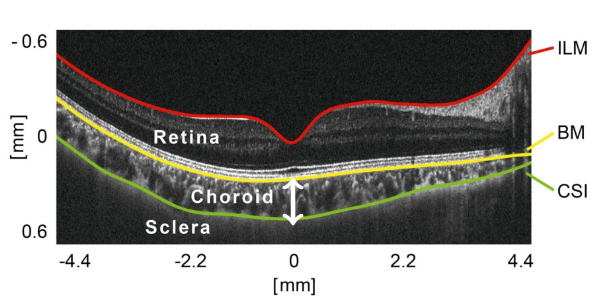
\includegraphics[width=1\textwidth]{./images/choroidalthickness}
    \caption{Choroidal thickness map and OCT B-scan with segmented layers \cite{Ronchetti2019statistic}}
    \label{fig:qc-layers}
\end{figure}

\section{Technical Background}

There are several approaches for detecting retinal boundaries, among them we can cite pixel intensity variations, texture analysis and graph search segmentation techniques. Pixel intensity variations are often used to calculate the total retinal thickness \cite{Alonso-Caneiro2013}, the method involves a series of processing steps where each pixel of the image is compared to a threshold chosen according to the color intensity of the pixels that contain the information about the location of the boundary \cite{Fabritius:09}. In the case of the ILM, it can be extracted easily because the vitreous body's pixels in the OCT scans are mostly black, while the membrane's pixels are mostly white. Therefore, taking the image from the top left corner, one can run a search algorithm that finds the first white pixel (the first that is over the threshold) from top to bottom and return its position. Running this same algorithm accros the $x$ axis will give us an array of pixels that can be smoothed by using cubic-spline interpolations that corresponds to the Internal Limiting Membrane (ILM). The process for extracting the Bruch's Membrane's (BM) inner-most layer is the same, since the sclera presents opaque pixels that can be omitted by the algorithm, the process would start from the bottom left corner and runs the algorithm from bottom to top until it reaches the Bruch's Membrane.      
\section{Results}
- Describe the data set
- Analyse implementation
\section{Conclusion}
\section{Future Work}
As the first step of our investigation, we have decided to algorithmically detect the retinal boundaries in order to give a mean value for its thickness measurement, this process can be error prone considering that a variation in intensity of the B-Scan pixels can introduce artifacts that would create irregularities on the final output. Therefore this controlled implementation will serve us as a base in order to annotate OCT scans and build a deep learning model that can perform the task of recognizing retinal boundaries on a more efficient way accross a higher number and varieties of scans allowing for a more flexible boundary detection. The model can be extended to detect the Choroid-Sclera Interface (CSI) potentially allowing to automate the choroid thickness measuring process, but it is important to take into consideration the lack of available experts in order to annotate the scans and the fact that it has been demonstrated that experts present inconsistencies when detecting the CSI even among identical images \cite{Ronchetti2019statistic} which may introduce biases in the deep learning model.  

\markboth{}{}

\newpage

\bibliographystyle{plain} % We choose the "plain" reference style
\bibliography{bibli} % Entries are in the "bibi.bib" file




\newpage
\thispagestyle{empty}
\markboth{}{}
  \normalsize
\begin{center}
\huge{\textbf{ Declaration of Independence}}\\[40mm]
\end{center}
\large
I affirm that the above work has been produced by myself without any unauthorized assistance and without the use of any other means than those indicated, and that I have marked as such all passages that have been taken literally or meaningfully from published or unpublished writings.\\[50mm]
Bienne, the \today

\newpage



\end{document}